
\begin{floatingfigure}[hr!]{4.5cm}
 \centering
         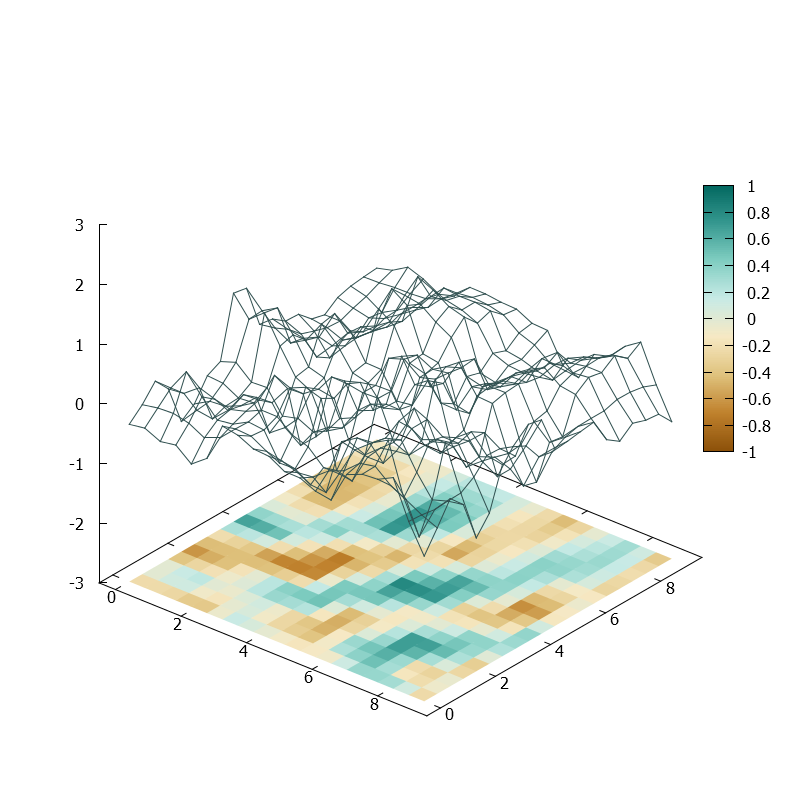
\includegraphics[width=7cm]{img/Plate0_A1.png}
         \caption[lorem]{Loren ipsum}
         \label{fig:Plate0_A1_}
\end{floatingfigure}
\lipsum[1-2]

\begin{figure}[ht!]
         \centering
         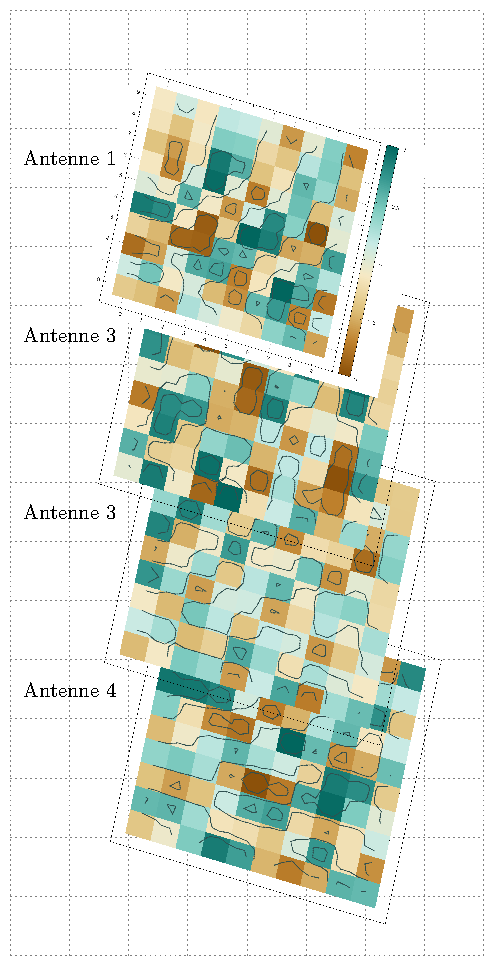
\includegraphics[width=0.7\textwidth]{img/complexitiy1.pdf}
         \caption[Reale Messwerte auf Kalibrierplatte]{Darstellung der Messwerte über eine Kalibierplatte ($1\times1$ Meter). In jeder Dimension wurden $10\times10$ Werte aufgenommen}
         \label{fig:Complexity1}
%
\end{figure}
%
\begin{figure}[ht!]
        \centering
        \begin{subfigure}[b]{0.3\textwidth}
            \centering
            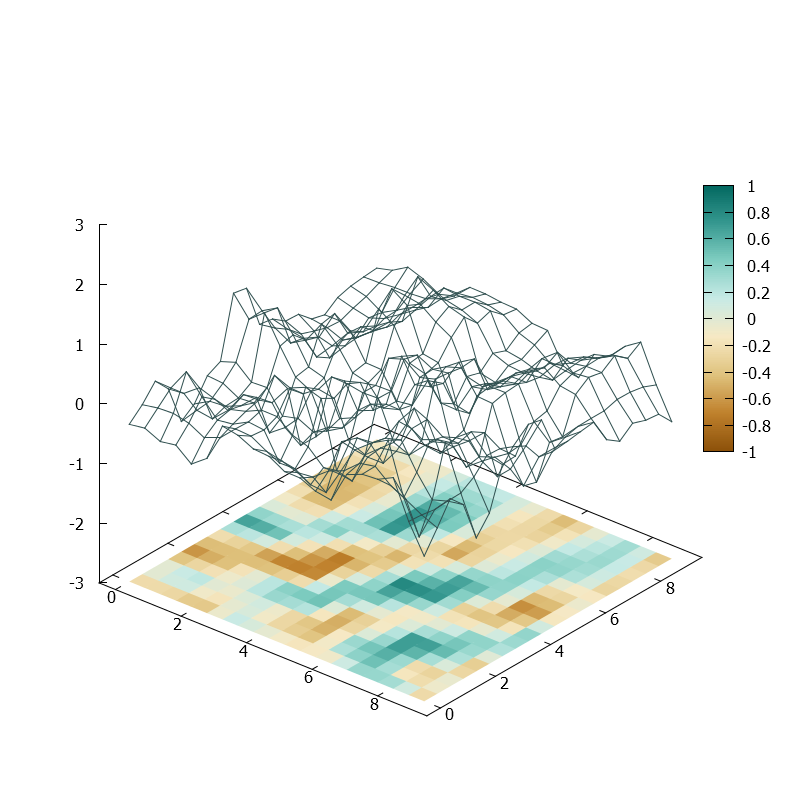
\includegraphics[width=\textwidth]{img/Plate0_A1.png}
            \caption[lorem]{Loren ipsum}
            \label{fig:Plate0_A1}
        \end{subfigure}%
         %add desired spacing between images, e. g. ~, \quad, \qquad etc.
          %(or a blank line to force the subfigure onto a new line)
        \begin{subfigure}[b]{0.3\textwidth}
            \centering
            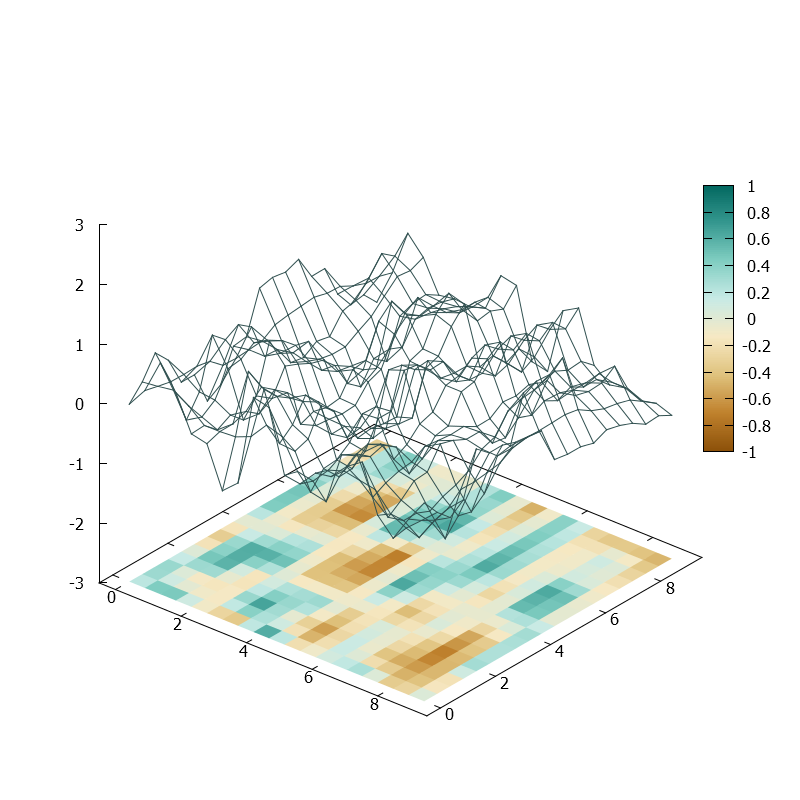
\includegraphics[width=\textwidth]{img/Plate0_A2.png}
          	\caption[Loren ipsum]{Loren ipsum}
         	\label{fig:Plate0_A2}
        \end{subfigure}
        %add desired spacing between images, e. g. ~, \quad, \qquad etc.
         %(or a blank line to force the subfigure onto a new line)
        \begin{subfigure}[b]{0.3\textwidth}
			\centering
			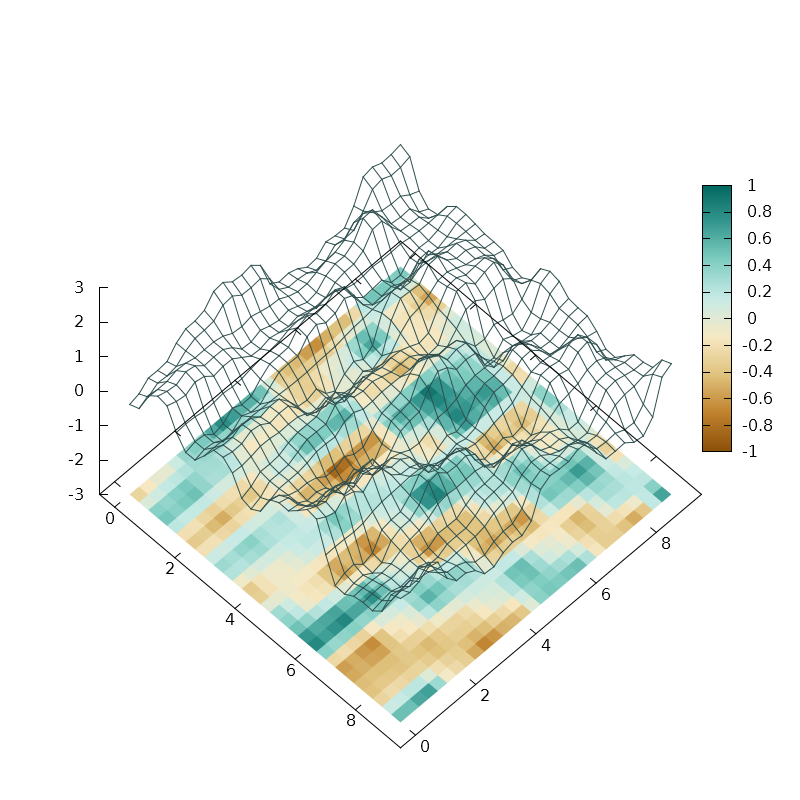
\includegraphics[width=\textwidth]{img/Plate0_A4.png}
			\caption[Loren ipsum]{Loren ipsum}
			\label{fig:Plate0_A4}
        \end{subfigure}
        \caption[Reale Messwerte visualisiert]{Die Komplexität des Problem kann anhand dieser Flächen abgeschätzt werden.}\label{fig:Real_Measurements}
\end{figure}
